\documentclass[11pt]{article}
%%%%%%%%%%%%%%%%%%%%%%%%%%%%%%%%%%%%%%%%%%%%%%%%%%%%%%%%%%%
%% package sillabazione italiana e uso lettere accentate
\usepackage[latin1]{inputenc}
\usepackage[english]{babel}
\usepackage[T1]{fontenc}
%%%%%%%%%%%%%%%%%%%%%%%%%%%%%%%%%%%%%%%%%%%%%%%%%%%%%%%%%%%%%

\usepackage{url}
\usepackage{xspace}
\usepackage{listings}
\usepackage{xcolor}
\usepackage{soul}

\usepackage[top=0.8in, bottom=0.8in, left=1in, right=1in]{geometry}

\makeatletter
%%%%%%%%%%%%%%%%%%%%%%%%%%%%%% User specified LaTeX commands.
\usepackage{manifest}

\makeatother

%%%%%%%
 \newif\ifpdf
 \ifx\pdfoutput\undefined
 \pdffalse % we are not running PDFLaTeX
 \else
 \pdfoutput=1 % we are running PDFLaTeX
 \pdftrue
 \fi
%%%%%%%
 \ifpdf
 \usepackage[pdftex]{graphicx}
 \else
 \usepackage{graphicx}
 \fi
%%%%%%%%%%%%%%%
 \ifpdf
 \DeclareGraphicsExtensions{.pdf, .jpg, .tif}
 \else
 \DeclareGraphicsExtensions{.eps, .jpg}
 \fi
%%%%%%%%%%%%%%%


\lstdefinelanguage{DDR}{
  keywords={System, Context, Robot, Event, EventHandler, Plan, stop, forward,
  backward, left, resumePlan, react, when, answerEv, handledBy, Actorm, for,
  task, Action, maxtime, val, ip, host, port, Actor, execAction, speed, angle,
  or, ->, time, right, println, photo}, keywordstyle=\color{blue}\bfseries,
  ndkeywords={class, export, boolean, throw, implements, import, this}, ndkeywordstyle=\color{darkgray}\bfseries, identifierstyle=\color{black},
  sensitive=false,
  comment=[l]{//},
  morecomment=[s]{/*}{*/},
  commentstyle=\color{purple}\ttfamily,
  stringstyle=\color{red}\ttfamily,
  morestring=[b]',
  morestring=[b]"
}

\lstdefinelanguage{DDRBASE}{
  keywords={RobotBase, Mainrobot, Magnetometer, Line, Distance, Motor,
  Rotation, Actuators, simulated, private, position, FRONT, BOTTOM, LEFT,
  RIGHTs}, keywordstyle=\color{blue}\bfseries, ndkeywords={class, export,
  boolean, throw, implements, import, this}, ndkeywordstyle=\color{darkgray}\bfseries,
  identifierstyle=\color{black},
  sensitive=false,
  comment=[l]{//},
  morecomment=[s]{/*}{*/},
  commentstyle=\color{purple}\ttfamily,
  stringstyle=\color{red}\ttfamily,
  morestring=[b]',
  morestring=[b]"
}

\newcommand{\java}{\textsf{Java}}
\newcommand{\contact}{\emph{Contact}}
\newcommand{\corecl}{\texttt{corecl}}
\newcommand{\medcl}{\texttt{medcl}}
\newcommand{\msgcl}{\texttt{msgcl}}
\newcommand{\android}{\texttt{Android}}
\newcommand{\dsl}{\texttt{DSL}}
\newcommand{\jazz}{\texttt{Jazz}}
\newcommand{\rtc}{\texttt{RTC}}
\newcommand{\ide}{\texttt{Contact-ide}}
\newcommand{\xtext}{\texttt{XText}}
\newcommand{\xpand}{\texttt{Xpand}}
\newcommand{\xtend}{\texttt{Xtend}}
\newcommand{\pojo}{\texttt{POJO}}
\newcommand{\junit}{\texttt{JUnit}}

\newcommand{\action}[1]{\texttt{#1}\xspace}
\newcommand{\code}[1]{{\small{\texttt{#1}}}\xspace}
\newcommand{\codescript}[1]{{\scriptsize{\texttt{#1}}}\xspace}

% Cross-referencing
\newcommand{\labelsec}[1]{\label{sec:#1}}
\newcommand{\xs}[1]{\sectionname~\ref{sec:#1}}
\newcommand{\xsp}[1]{\sectionname~\ref{sec:#1} \onpagename~\pageref{sec:#1}}
\newcommand{\labelssec}[1]{\label{ssec:#1}}
\newcommand{\xss}[1]{\subsectionname~\ref{ssec:#1}}
\newcommand{\xssp}[1]{\subsectionname~\ref{ssec:#1} \onpagename~\pageref{ssec:#1}}
\newcommand{\labelsssec}[1]{\label{sssec:#1}}
\newcommand{\xsss}[1]{\subsectionname~\ref{sssec:#1}}
\newcommand{\xsssp}[1]{\subsectionname~\ref{sssec:#1} \onpagename~\pageref{sssec:#1}}
\newcommand{\labelfig}[1]{\label{fig:#1}}
\newcommand{\xf}[1]{\figurename~\ref{fig:#1}}
\newcommand{\xfp}[1]{\figurename~\ref{fig:#1} \onpagename~\pageref{fig:#1}}
\newcommand{\labeltab}[1]{\label{tab:#1}}
\newcommand{\xt}[1]{\tablename~\ref{tab:#1}}
\newcommand{\xtp}[1]{\tablename~\ref{tab:#1} \onpagename~\pageref{tab:#1}}
% Category Names
\newcommand{\sectionname}{Section}
\newcommand{\subsectionname}{Subsection}
\newcommand{\sectionsname}{Sections}
\newcommand{\subsectionsname}{Subsections}
\newcommand{\secname}{\sectionname}
\newcommand{\ssecname}{\subsectionname}
\newcommand{\secsname}{\sectionsname}
\newcommand{\ssecsname}{\subsectionsname}
\newcommand{\onpagename}{on page}

\newcommand{\xauthA}{Roberto Casadei }
\newcommand{\xauthB}{Massimiliano Martella}
\newcommand{\xauthC}{Roberto Reda}
\newcommand{\xfaculty}{II Faculty of Engineering}
\newcommand{\xunibo}{Alma Mater Studiorum -- University of Bologna}
\newcommand{\xaddrBO}{viale Risorgimento 2}
\newcommand{\xaddrCE}{via Venezia 52}
\newcommand{\xcityBO}{40136 Bologna, Italy}
\newcommand{\xcityCE}{47023 Cesena, Italy}

\definecolor{myrgb}{RGB}{0, 0, 100}
\newcommand{\mycolor}{myrgb}
\definecolor{violet}{RGB}{150, 0, 100}
\definecolor{red}{RGB}{250, 0, 0}
\definecolor{green}{RGB}{0, 250, 0}
\definecolor{blue}{RGB}{0, 0, 250}
\definecolor{lightblue}{RGB}{200, 210, 240}

\usepackage{float}

\usepackage{color}
\newcommand{\colorize}[1]{{\color{\mycolor}#1}}
\newcommand{\redize}[1]{{\color{violet}#1}}
\newcommand{\red}[1]{{\color{red}#1}}
\newcommand{\green}[1]{{\color{green}#1}}
\newcommand{\blue}[1]{{\color{blue}#1}}
\newcommand{\lightblue}[1]{{\color{lightblue}#1}}

\newcommand{\myquote}[1]{
\setlength{\leftskip}{3cm}

\noindent \emph{#1}

\setlength{\leftskip}{0pt}
}

\usepackage{tikz}
\usepackage[english]{babel}
\usepackage{blindtext}
\newcommand{\mybox}[2]{%
         \begin{center}%
            \begin{tikzpicture}%
                \node[rectangle, draw=#2, top color=lightblue, bottom
                color=lightblue, rounded corners=5pt, inner xsep=5pt, inner
                ysep=6pt, outer ysep=10pt, line width=1.8pt]{
                \begin{minipage}{.90\linewidth}#1\end{minipage}};%
            \end{tikzpicture}%
         \end{center}%
}


\newcommand{\quindi}[1]{\blue{\emph{$\Rightarrow$ #1}}}
%
% Comments
%
%%% \newcommand{\todo}[1]{\bf{TODO:}\emph{#1}}

\begin{document}

\title{Software Systems Engineering\\
	Final project process report}

%%% \author{\xauthA \and \xauthB}
\author{\xauthA \and \xauthB \and \xauthC}


%\institute{%
%%%  \xunibo\\\xaddrCE, \xcityCE\\\email{\{nameA.studentA, nameB.studentB\}@studio.unibo.it}
%  \xunibo\\\xaddrCE, \xcityCE\\\email\ roberto.casadei12@studio.unibo.it
%}

\maketitle

%% \begin{abstract}
%% \footnotesize
%%This a Latex template to be used for the reports of Software Engineering.
%%\keywords{Software engineering, managed software development, reports, ....}
%%\end{abstract}

%%% \sloppy

%===========================================================================
\section{Introduction}
\labelsec{intro}
%===========================================================================

 This report represents a concise, informative, and annotated \textbf{snapshot}
 of the final project for the course
  ``Software Systems Engineering'' at Alma Mater Studiorum - University of
  Bologna.

%===========================================================================
\section{Vision}
\labelsec{Vision}
%===========================================================================

\subsubsection*{Product and process}

We believe that a good software product is the natural result of a
\emph{mature, systematic process} that, as such, should be repeatible, defined,
managed and -- if we make it -- even optimizing (see \emph{Capability Maturity
Model}).


\subsubsection*{Why $\Rightarrow$ What $\Rightarrow$ How}

\emph{We believe that there is no code without design, no design without
analysis, no analysis without requirements.} So, we recognize the causal
progression from the \emph{why} (vision/goals/requirements) to the \emph{what}
(analysis) and finally to the \emph{how} (design/code).


\subsubsection*{Projects and knowledge}

Software projects are inherently \textbf{knowledge-intensive}. 
  As such, we think it is prominent to look for better ways to:
  
\begin{itemize}
  \item \emph{Make project knowledge \textbf{explicit}} (cf. project artifacts,
  their documentation, and the documentation about their craft)
  \item \emph{Make project knowledge accessible, searchable, navigable, \ldots
  }(cf. project websites, wikis, issue tracking systems, \ldots)
  \item \emph{Keep the information \textbf{consistent}} (cf. editing of
  different representations of the same resource, the relationship between analysis and
  design artifacts)
  \item \emph{\textbf{Link} related information} (cf. traceability)
  \item \emph{Keep track of changes} (cf. version control, continuous
  testing/build/delivery systems)
  \item \ldots
\end{itemize}

\subsubsection*{Make the best out of analysis}

We recognize the importance of analysis for a mature process, but we don't want
to waste time by just producing informal knowledge. 
Instead, we would like to \emph{capitalize the
effort spent in analysis by producing something that has value, that is, 
working software (prototype) and reusable frameworks}.


\subsubsection*{Reuse}

We believe that \emph{reuse} is prominent in what we do because it is 
 \emph{the key to efficiency and effectiveness}, to productivity and quality.

Reuse can happen at several levels and forms, but we are ultimately interested
in \emph{code reuse}.


\subsubsection*{Starting from problems: top-down approach}

We firmly believe that the results from (requirements and problem) analysis
should NOT depend on the reference paradigm and, least of all, on the technological platform. 

Thus, we strive to follow a \emph{top-down approach}, that is, from the problem
to the technology.

 We are aware that paradigms (and, in general, the conceptual spaces
 projected by a given technology) are similar to \emph{lens} that make certain
 aspects clearly visible while completely hiding others. This is not bad,
 because \textbf{complex systems} typically consists of multiple
 \textbf{(orthogonal) dimensions}, and each dimension might require different 
 (conceptual and practical) tools to be adequately investigated.
 
 As a consequence, we think that, in order to be able to effectively tackle the
 problems at hand, we should
 
 \begin{enumerate}
   \item be aware of the limitations of adopting a single point of view
   \item be aware of the current reference conceptual space in use and 
   \item try to find and use the (conceptual) tools that most fit the problem
 \end{enumerate}
 
 so that we can reduce both the cognitive load and the abstraction gap (if a
 platform exists or can be built).


\subsubsection*{Abstraction gap and innovation}

By following a top-down approach, we constantly \textbf{evaluate
the abstraction gap} in order to gain a better vision of what we need to
\emph{effectively} build the kind of systems we are considering and also as a
way to \emph{innovate}.

\myquote{The entire history of software engineering is that of the rise
in levels of abstraction. -- Grady Booch}

\subsubsection*{Systemic approach for tackling complexity}

As we are dealing with (complex) software systems, we believe
that a \textbf{systemic approach} fits more than an algorithmic approach and 
gives us access to more powerful conceptual tools.


\subsubsection*{Reflection and continuous improvement}

We think that the key for effectiveness lies in a continuous, \textbf{critical
analysis} of the problems we encounter, the solutions we advance, and the
approach we follow for mapping the former to the latter. A question we should
always ask ourselves is: \emph{what are we doing and why?}

We explicitly focus on \textbf{relationships between the conceptual tools used
in a project and the project itself} (i.e., processes and artifacts).

We think that the use of the right tools can help minimizing
 the \emph{accidental complexity}, thus allowing us to \textbf{focus on the
 essential complexity} of our systems. 
 
 
\subsubsection*{Long-term vs. short term productivity} 
 
 We believe that the \textbf{trade-off}  \emph{between
 long-term and short-term productivity} should be guided (at least) by the potential for
 reuse and the lifetime of the software artifacts produced. In this view,
 addressing the abstraction gap is key to grow and optimize in a sustainable
 manner.

\subsubsection*{Human factors in software projects}

We are conscious that software development is a \emph{human activity} and
many issues arise from the coordination of several human players with
different character, skillset, expectations, \ldots

\myquote{Most software project problems are sociological, not technological. --
From 'Peopleware' \cite{peopleware}}

This is why we need to follow a \textbf{disciplined approach} (enforced by
rules, processes and tools), while being aware that people require comfort and 
space for expressing themselves through creativity, responsibility, trial and error, \ldots

\subsubsection*{Collaborative approach}

Our work approach should be \textbf{cooperative} (rather than
\emph{competitive}).

The contracts and boundaries of software components should be defined up-front,
  so that the work can be parallelized across many people. In this view, the
  analysis is crucial (and, in particular, the logic architecture).
  
Moreover, the use of version control tools such as \emph{git} is paramount to 
  effectively carry out collaborative software development efforts. Again, 
  tools have to be used with discernment and thought (cf. Git flow
  \cite{gitflow}).



\subsubsection*{Thus\ldots}

We think that a software development process built upon the
principles outlined above can maximize the value of the effort spent
during analysis and development, effectively produce software architectures that
are resistant to requirements change, and even turn those changes into an
opportunity to increase the organizational know-how.


% TRACEABILITY

% WHY -> WHAT -> HOW

%===========================================================================
\section{Goals}
\labelsec{Goals}
%===========================================================================

 We use this final project as an opportunity to actualize the vision.\\

\subsubsection*{Product and process}

The main goal is to focus on the \textbf{relationships between the software
production process and the final product}, with particular attention on the
\textbf{artifacts produced in the phases of requirements and problem analysis}.

\subsubsection*{Project agility}

Another main goal is to test \textbf{how much the project is resistant to
changes in requirements}. What is the impact of required monotonic extensions 
on a product whose production is based on 'formal', 'technology independent'
artifacts?

\subsubsection*{Reuse of domain knowledge}

We are aware that the system we are building is just one of the countless
applications that could be built in this domain. So, we generalise/abstract from
the issues we encounter in a sustainable manner, so that we can \textbf{factor
domain-knowledge out of the specific system}.

\subsubsection*{Incremental prototyping}

By analyzing the requirements and the problem, we would like to produce a
\textbf{working prototype by following an incremental (\emph{piecemeal growth})
approach}.

\subsubsection*{Agile vs. model-driven}

We have the goal to compare and keep the best from both agile and model-based approaches.

%In particular, we would like to evaluate the cost of passing from a
% homogeneous, concentrated system to a distributed, etherogeneous system.

\subsubsection*{MDSD, software factories, meta-models, DSLs, and XText}

We would like to factor the effort spent in filling the abstraction gap out into
 reusable artifacts. 
We think that an effective way to do so consists in building \textbf{custom
 meta-models} and associated \textbf{code generators}.
XText helps us in this job by establishing a \emph{link between models and
code} (through the automatic meta-model inference from the DSL grammar).

In other words, we strive to incrementally build, around a \emph{DSL}, a
\textbf{software factory} -- through a continuous collaboration between application
designers and system designers -- that encapsulates the knowledge to pass from ``what'' to ``how''.

With such an approach
\begin{itemize}
  \item we make the conceptual space of our framework/DSL explicit
  \item we create a common language (cf. \emph{ubiquitous language} in DDD)
  between (business experts and) application designers and system designers
  \item we can express not only design models, but
  even analysis models (e.g., declaratively stating what emerges from the
  problem)
\item we have a direct, explicit, and
  automatic link from analysis/design elements to implementation elements
\end{itemize}

A DSL represents an organizational asset, the
synthesis of the organizational know-how in a domain.

Moreover, we underline that there is even more benefit in \emph{building} a DSL
rather than \emph{using} it. In fact, it is key for rapid prototyping and for
systematically pointing out the abstraction gap by fostering a top-down
approach.


\subsubsection*{While correlating what we do with the following concepts}

\begin{itemize}
  \item Models ($\Rightarrow$ Structure, Interaction, Behavior) as a way to
  capture the essential characteristics of what we talk about
  \item Software reuse as the key element to deal with bounded resources
     \begin{itemize}
       \item Pattern vs. library vs. framework vs. middleware vs. DSL
	 \end{itemize}
  \item Technologies as specific ways to actualize designs but also as
  conceptual spaces (i.e., ``representing'' a paradigm)
  \item Logic architecture as the main result from analysis and possibly our
  main specification of the problem at hand
  \item Traceability (from requirements to architecture to code) as a way to
  support ``informational consistency'' within the project
  \item Specific vs. schematic vs. generic parts of software
\end{itemize}

% How do the project phases (analysis, design, ..) change when the
%reference paradigm/technology-hypothesis changes?

% (long-term) advantage that results from building frameworks that
%adequately fill the abstraction gap that had been identified

% systematic comparison


\newpage
%===========================================================================
\section{Requirements}
\labelsec{Requirements}
%===========================================================================

\mybox{The requirements are copied literally.}

\subsection{STEP 1}

Design build a (prototype of a) software system that:
\begin{itemize}
\item allows a differential drive robot to move in autonomous way from a
prefixed point \redize{A1} to a prefixed point \redize{A2} under a set of
assumptions on the external environment (e.g. plain roof, no obstacle, etc) 
\item emits a signal named  \redize{<RobotName>Enter} when the robot enters into
a SensibleArea delimited by a black line and 
a signal named  \redize{<RobotName>Exit}
when the robot exits from the area 
\item allows the robot to react (as soon as possible) to a
 \redize{halt} command sent by
the user (via a remote console)
\end{itemize}

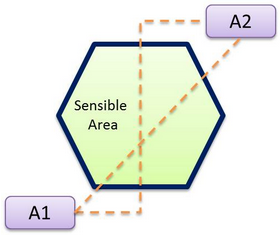
\includegraphics[scale=0.6]{img/reqImg.png}

\subsubsection{Non functional requriments at step1}.

The main goal is not only to satisfy the functional 
reuirements but it is mainly related to the relationships 
between the software production process and the final product, 
with particular attention on the artifacts produced in the phases 
of requiremt and problem analysis

\subsection{STEP 2}

 \redize{After} the development of this prototype, consider the possibility 
to enhance the functional capabilities of the robot, by allowing it :
\begin{itemize}
\item to perceive an obstacle within the  \redize{SensibleArea} amd, once the
obstacle is detected:
\begin{itemize}
  \item to execute some alternative behavior (in term of moves)
  \item (optionally) , to use a webcam to take a picture of the obstacle and to
  send it to some user command console and/or to use some device 
  to emit sounds or vocal alerts
\end{itemize}
\end{itemize}

\subsubsection{Non functional requriments at step1}

The main goal is yo discuss how some change (monotonic extensions) 
of the requirements imact on a product whose production is based on 'formal', 
'technology independent' artifacts.


 
 
 
 \newpage
%===========================================================================
\section{Requirement analysis}
\labelsec{ReqAnalysis}
%===========================================================================

\subsection{Basic Requirements Analysis}

\mybox{
We are aware of the \textbf{limitations of producing informal artifacts} 
 (such as the glossary, use cases, etc). However, we consider them as 
 intermediate steps that help us to reach a basic, high level
 \textbf{understanding} of the problem before we start drawing formal models
 from the informal requirements.
 }

\subsubsection{Elements to be understood/defined}

\mybox{
First of all, the requirements are attentively read. As a rule of thumb,
\textbf{nouns} point out the entities of the problem, \textbf{verbs} suggest
what these entities should do, and \textbf{adverbs}/\textbf{adjectives} work as
modifiers and suggest properties.
}

Step 1:

\begin{itemize}
  \item \green{Differential drive} \blue{robot}
  \item The robot should be able to \red{move} \green{autonomously} from
  \green{prefixed} \blue{point} to \green{prefixed} \blue{point} (in space)
  \item Assumptions on the external \blue{environment}
  \item The robot \red{emits} a \green{named} \blue{signal} when it
  	\red{enters}/\red{exits} a
  	\blue{sensible area} \green{delimited by a black line}
  \item The robot should be able to \red{react} \green{as soon as possible} to a
  	\texttt{halt} \blue{command} \red{sent} by the \blue{user} (via a
  		\green{remote} \blue{console})
\end{itemize}

Step 2:

\begin{itemize}
  \item The robot should be able to \red{perceive} an \blue{obstacle} within the
  sensible area
  \item When the obstacle is \red{detected}, the robot should \red{execute} some
  	\green{alternate} \blue{behavior} (in term of \blue{moves})
  \item and \red{use} a \blue{webcam} to take a \blue{picture} and to \red{send}
    it to some \blue{user command console} and/or to use some \blue{device} to 
    \red{emit} \blue{sounds} or \blue{vocal alerts} 
\end{itemize}

The aforementioned elements have to be defined \textbf{formally} and
\textbf{unambiguously}.

%Moreover, as we are in the domain of \textbf{Robotics and Internet of Things}, 
%  we should look for \textbf{generalizations} or, if those have an overwhelming
%  impact for the moment, at least avoid to preclude such a prospect in the
  % future.
  
\subsubsection{Questions \& Answers}

\mybox{As \textbf{requirements are ambiguous, incomplete}, etc. we ask the
customer some questions.}

Questions to the customer:

\begin{itemize}
%  \item What is a \emph{robot}?
%  \item Should be consider only \emph{differential drive} robots?
  \item What means that the robot moves \emph{autonomously}? \\
  \emph{$\Rightarrow$ When the robot is turn on, it starts to move without being
  remotely controlled.}
  \item What's the starting point and the final point? \\
  \emph{$\Rightarrow$ The starting point is the place in which the robot is
  initially placed and the final point is where the robot stops.}
%  \item What is the robot supposed to do when it receives the Halt command
  \item What is a \emph{signal}? What means it is \emph{emitted} --
  	\emph{where}, \emph{to who}?
  \item What is a \emph{command}? Where do they originate from? 
  \item What is, in general, a \emph{sensible area}?
  \item \ldots\ldots\ldots\ldots\ldots
%  \item How do the remote console \emph{communicate} with the robot? What
% semantics? In what language?
\end{itemize}


%From the requirements, the interactions with the customer, and some
%generalisation, it follows that a robot is an entity that:

%\begin{itemize}
%  \item is able to \emph{sense} the environment through \emph{sensors}
%  \item is able to \emph{execute commands} (possibly \emph{acting} on the
%  environment through \emph{actuators})
%\end{itemize}

%If we consider a robot as such, it must exist another entity -- which
%we call its \emph{mind} -- that sends commands to the robot. The mind can 
% run on the same computational support of the robot (\emph{embedded mode}) or
 % on a different computational node (\emph{avatar mode}).
 

\subsubsection{Use Cases}

\mybox{A very high-level, user-centered representation of functional
requirements.}

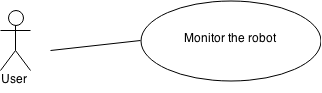
\includegraphics[scale=0.6]{img/ISS-final-UseCase.png}

\subsubsection{Scenarios}


\begin{itemize}
  \item \textbf{Scenario 1: Basic scenario} \\
	Actors
	\begin{itemize}
	  \item The robot
	  \item The user
	\end{itemize}
	
	Description
	
	\begin{itemize}
	  \item 	The user monitors the robot. The robot starts
	   to move autonomously.
	   The user triggers the Halt signal through the
	   console. The robot stops.
	\end{itemize}
\end{itemize}

 
 
\subsubsection{The system}

\mybox{ 
As we are following a \textbf{systems approach}, first of all we look for
the \textbf{subsystems}.
}
 % and try to ``draw a line around our system'' in order to
 %define its \textbf{boundaries}.
 
From the requirements, it follows that the system consists in the following
subsystems:

\begin{itemize}
  \item The robot
  \item The remote console of the user
\end{itemize}
 
As the console is remote, it follows that the system is \textbf{distributed}. 

%\subsubsection{Communication}

%The robot interacts with the mind and the remote console via \emph{message
%passing}, i.e., by receiving and sending \emph{messages}. Such communications
%are \emph{point-to-point} and their semantics is the same as defined in the
%QActor framework.

%\subsubsection{Signals}

%Signals are communication acts with no defined recipient, but rather they are
%emitted to the environment.

%The semantics of a signal is the same as the semantics of an \emph{event} as
%defined in the QEvent framework. The entity that emits an event is known as an
% \emph{event source}. An entity can perceive an event if it is \emph{interested}
% in that kind of event.

% Events and streams



\subsection{Domain Model}

\mybox{For us, a \textbf{model} is characterized by three key dimensions:
\begin{enumerate}
  \item Structure
  \item Interaction
  \item Behavior
\end{enumerate}

In order to express these models formally, we use (Java) interfaces and 
  (JUnit) test plans. This is a convention used in our software house.
}

\mybox{In our software house, we have already analyzed -- in past projects --
many of the concepts that emerge from requirement analysis, namely:

\begin{itemize}
  \item Base robot
  \item Robot component
  \item Robot command
  \item Sensor
  \item Event
\end{itemize} 

In other words, we exploit the domain models that have been built 
 during the past projects in this very domain.
}

\subsubsection{Base Robot}

\mybox{
Structure

\begin{itemize}
  \item A base robot is a \emph{composed} entity
  \item It consists of a set of \emph{robot components}, for example:
  \begin{itemize}
    \item \emph{Sensors}, which allow it to sense the world around it
    \item \emph{Actuators}, which allow it to act on the world around it
  \end{itemize} 
\end{itemize}

Interaction

\begin{itemize}
  \item By perceiving and raising \emph{events}
  \item An entity can ask a base robot to \emph{execute} a \emph{command}
\end{itemize}

Behavior

\begin{itemize}
  \item Passive
\end{itemize}
}


See:
\begin{itemize}
  \item \texttt{it.unibo.iot.executors.baseRobot.IBaseRobot}
  \item \texttt{it.unibo.iot.robotComponent.IRobotComponent}
\end{itemize}



\subsubsection{Autonomous robot}

\mybox{ 
An autonomous robot cannot be commanded/controlled externally.

With respect to a base robot, an autonomous robot cannot be requested to execute
commands, that is, it has an autonomous behavior.

%Structure

%\begin{itemize}
%  \item An autonomous robot is s composed entity.
%  \item It consists in a \emph{base robot} and a \emph{mind}.
%\end{itemize}

%Interaction

%\begin{itemize}
%  \item By perceiving and raising \emph{events}.
%\end{itemize}

%Behavior

%\begin{itemize}
%  \item Autonomous
%\end{itemize}

%Note that the \emph{mind} can run on the same computational support of the
% robot or on a different computational node. 
%In the first case we say the robot is controlled in Embedded-mode, 
% while in second case we say that the robot is controlled in Avatar-mode.
%In the latter case, the robot is a distributed system and communication happens
% via message passing.
}


%\begin{itemize}
%  \item By \emph{message-passing} (according to the semantics of the QActor
%  framework)
%  \item By perceiving and raising \emph{events} (according to the semantics of
%  the QEvent framework)
%\end{itemize}

\subsubsection{Commands} %, plans

\mybox{
A \emph{command} is a passive entity characterized by a (textual)
representation.

A \emph{timed command} consists in a command and a \emph{duration}.

Note: this is \textbf{not} what, in the requirements, the term ``command''
refers to.

%A \emph{plan} is a sequence of commands.
}

See:

\begin{itemize}
  \item \texttt{it.unibo.iot.models.commands.ICommand}
  \item \texttt{it.unibo.iot.models.commands.baseRobot.IBaseRobotCommand}
  \item \texttt{it.unibo.robotUsage.interpreted.IRobotTimedCommand}
\end{itemize}

\subsubsection{Sensors, Actuators}

\mybox{
A \emph{sensor} is an \emph{observable} (cf. pattern Observer \cite{gof94})
robot component which provides a \emph{value} of a certain \emph{type}.

Conversely, an \emph{actuator} is an entity that can execute \emph{commands} of
a certain \emph{type}.

Note that sensors and actuators have physical counterparts, but we focus on
their software representatives. }

\begin{itemize}
  \item \texttt{it.unibo.iot.sensor.ISensor}
  \item \texttt{it.unibo.iot.executor.IExecutor}
\end{itemize}

$$\\$$

$$\\$$

NOTE: After problem analysis and in general after process iterations, other
concepts are integrated into the domain model.



\newpage

The following UML diagrams provide an excerpt, an integrated overview of the
concepts that have been modelled in the past by our software house.

\begin{figure}[H]
    \centering
     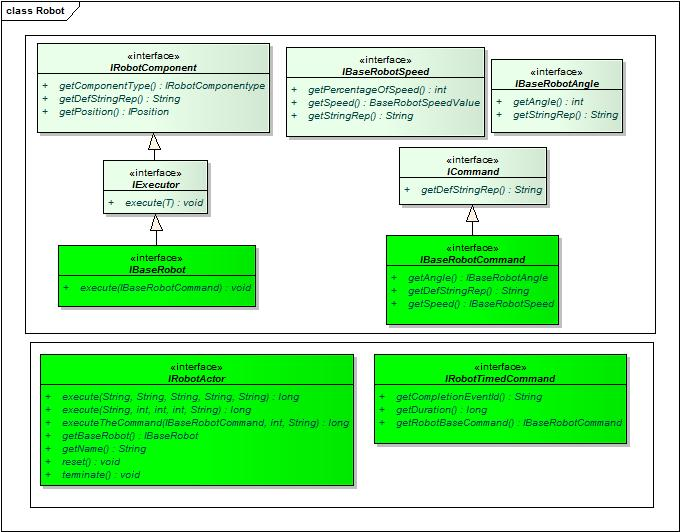
\includegraphics[scale=0.80, trim=2cm 0 0
     -1cm]{img/RobotModel.jpg}
\end{figure}

\begin{figure}[H]
    \centering
     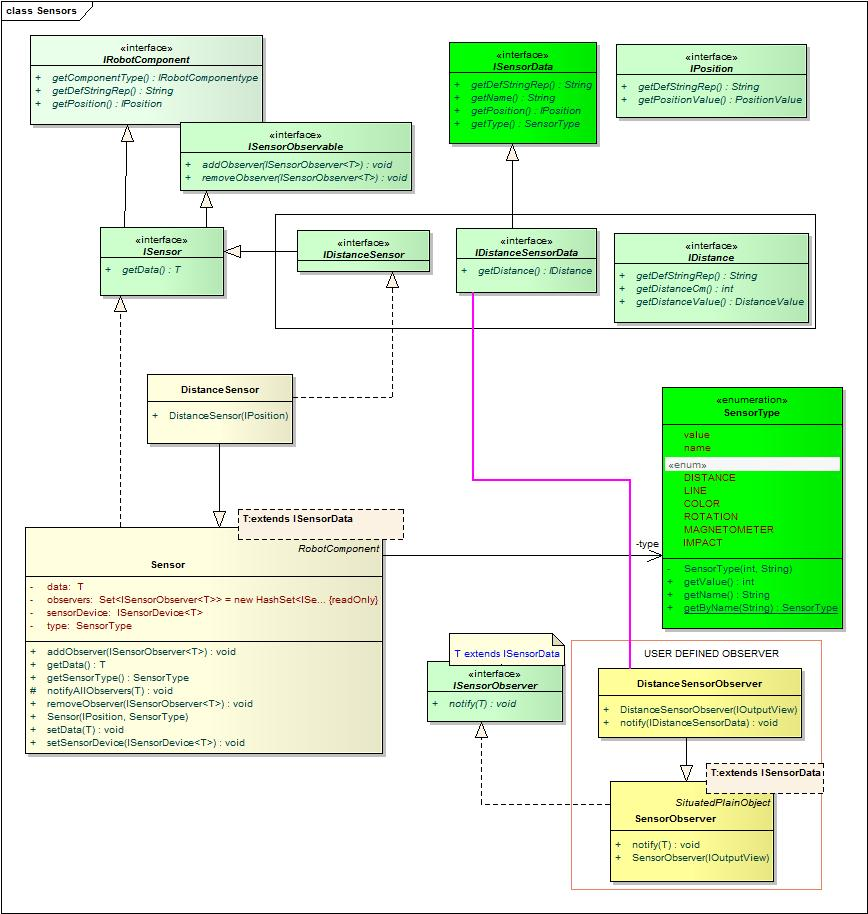
\includegraphics[scale=0.68, trim=3cm 0 0
     -1cm]{img/SensorsModel.jpg}
\end{figure}

\\

\\

%\mybox{Note: many of the concepts that will be introduced in section ``Problem
%Analysis'' will be integrated in the domain model.}


%We follow a \emph{systemic approach}. From the requirements, it follows that
% the system is structurally composed of three \textbf{subsystems} (for which we already know the deployment,
%see the Deployment section \ref{sec:Deployment}), \colorize{as expressed by the
%following textual, formal model (specification):}
 
\lstset{frame=single, language=java, breaklines=true, numbers=left,
basicstyle=\fontfamily{pcr}\selectfont\footnotesize\color{black},
    keywordstyle=\color{blue}\bfseries,}
    
%\begin{lstlisting}
%context( ctxofbutton, "Address1",  "Protocol1", "Port1" ).
%context( ctxofcontrol,   "Address2", "Protocol2",  "Port2" ).     
%context( ctxofled,   "Address3", "Protocol3",  "Port3" ).      
%\end{lstlisting}

%\colorize{where subsystems are modelled as \emph{contexts}. The addresses, the
%protocols, and the ports will be specific to a particular system deployment
%(Note that other means for specifying the distribution configuration might be
%used -- they are unessential at this level).

%We recur on the structural dimension.
%We also know what \textbf{components} the system is composed of, and how they
% are distributed in the aforementioned subsystems.}





\newpage
%===========================================================================
\section{Problem analysis}
\labelsec{ProblemAnalysis}
%===========================================================================

\subsection{Basic problem analysis}

\mybox{Here, we analyze the problem in a systematic manner. 
  We strive to \textbf{express our ponderings through incontrovertible
  evidence}.
  
  As an approach, we start off by considering the parts of the system, their
  behavior, and how they interact with each other. Then, we \textbf{zoom} into
  them, looking for problems at each level. }

%\mybox{Summary of concepts covered:
%\begin{itemize}
%  \item Physicality
%  \item Situatedness
%  \item Etherogeneity
%  \item Environment representation
%  \item Situated action
%\end{itemize}
%}

\subsubsection{The application}

  From the requirement analysis, we know that the \emph{system} is composed of
  \textbf{two parts}: a robot and a (remote) user console.
  
  Usually, these two parts are on different computational nodes (i.e., the
  system is \emph{distributed}) and must be able to
  \textbf{communicate over a network} (such as a wireless network).
    
  The console must be able to emit information units, whereas the robot must be
  able to perceive them and react to them with some behavior.   
  Note that we focus on the ``information flow'' but we do not want to
    over-commit towards a specific communication mechanism.
  
\subsubsection{The robot}  
  
  A robot consists of many \emph{robot components} (such as sensors, actuators,
  \ldots).
    Each \emph{type of sensor} (or actuator) is potentially different from one
    another in respect to its physical configuration, the values it provides, the
    rate of its working cycle, etc\ldots .
  
\begin{figure}[H]
    \centering
     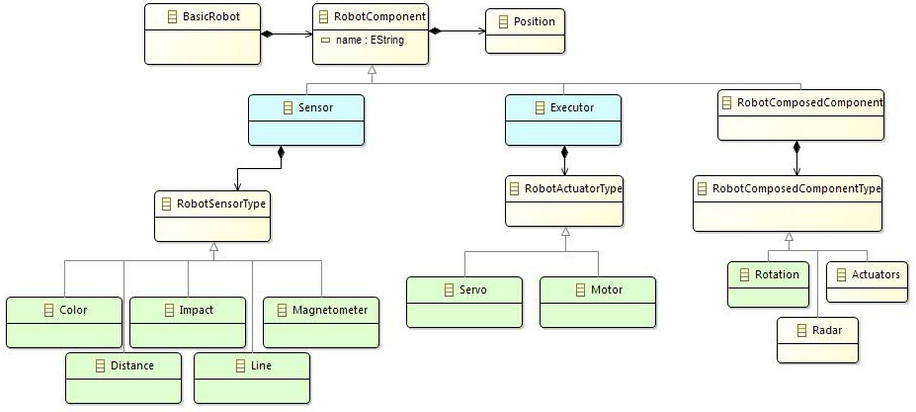
\includegraphics[scale=0.60, trim=4cm 0 0
     -1cm]{img/concept_baseRobot.png}
    \caption{A base robot.}
    \label{fig:baserob}
\end{figure}  

  About the ``\emph{origin of the robot's behavior}'', we note that a robot can
  be ``executed'' in (at least) two main \emph{modes}:
\begin{itemize}
  \item \emph{avatar-mode}: the robot is controlled by an external entity
  (the \emph{mind})
  \item \emph{planned-mode}: the robot is not externally controlled; instead, it
  executes a built-in behavior (see more about that later)
\end{itemize}
  
  Applications require the robot to be able to carry on multiple activities
  (logically) at the same time, such as:
  
\begin{itemize}
  \item Move in some direction (or, in general, command one or more actuators)
  \item Look for and react to sensor and application events
  \item Execute asynchronous activities (consider the case for making a video)
  \item \ldots
\end{itemize}
  

\subsubsection{Physicality, situatedness, and environment}

The \textbf{physical robot} is \textbf{situated} in the real world, can perceive
it via sensors, and can act upon it via actuators. Similar considerations apply
to the software robot. 

We also note that the notion of \textbf{environment} is prominent
in this domain.


\subsubsection{Etherogeneity of robots}

We also note that, in the real world, robots are usually
\textbf{etherogenous} (built with different hardware/firmware/software
components and configurations). 

As a consequence, it's advisable to build the software system in a
\textbf{technology-independent way} and to make the configuration procedure
automatic.

 
\subsubsection{Physical robot configuration/deployment}

As robots can be physically built in different and etherogeneous ways, 
 we should be able to easily deploy our robot software system to different
 physical embodiments.


\subsubsection{Autonomy, agency, proactivity} 
 
  Robots are oriented to \emph{action}. Thus, autonomous robots are
  \emph{agents}. As agents, they are \emph{proactive} because the 
  criterion for deciding what to do must be internal.

\subsubsection{The environment is dynamically unknown, unpredictable}

The sequence of elementary steps of the robot behavior \emph{cannot be entirely
defined offline}, because the environmental dynamics cannot be always anticipated. 
 
 
\subsubsection{Plans}
 
 We note that, in the literature, the problem of ``accomplishment of prolonged,
 complex, and dynamically changing tasks in the real world'' has been tackled
 by (among the others) \textbf{plan-based approaches} to robot control.

 We also note that plans represent the application of the
 \emph{divide-et-conquer} principle to the need of giving structure to
 (robot) behavior.
 
 A \emph{plan} is defined as a sequence of plan actions (moves).


\begin{figure}[H]
    \centering
     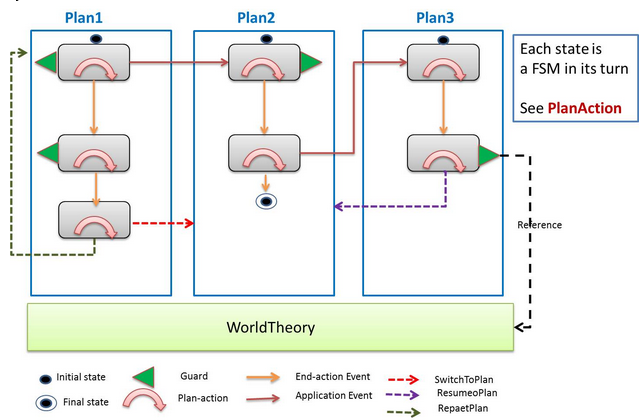
\includegraphics[scale=0.60, trim=4cm 0 0
     -1cm]{img/concept_plan.png}
    \caption{Plans.}
    \label{fig:plans}
\end{figure}  


\subsubsection{Actions, moves}

An \emph{action} represents a (high-level) abstraction upon what a robot can do.

A \emph{move} is a built-in action (e.g., move towards, take a photo, \ldots).

A \emph{plan action} is a \emph{guarded}, \emph{timed} move that can be executed
while also reacting to events.

\begin{figure}[H]
    \centering
     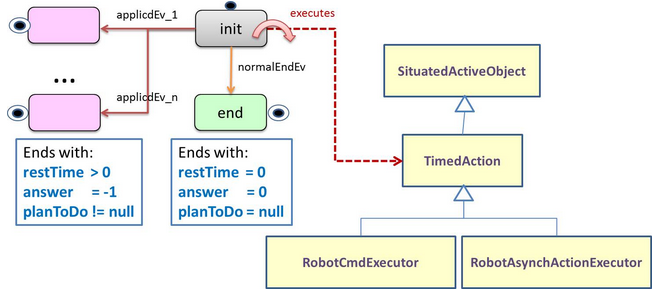
\includegraphics[scale=0.60, trim=4cm 0 0
     -1cm]{img/concept_planAction.png}
    \caption{Plan actions.}
    \label{fig:planActs}
\end{figure} 


Moreover, actions can be:

\begin{itemize}
  \item \emph{synchronous} -- i.e., the action must be completed before
  executing the next move
  \item \emph{asynchronous} -- i.e., the action starts but the robot can
  immediately execute the next move
\end{itemize}

Actions could be \emph{interruptible}.

 
\subsubsection{Environment and representation}

The importance of the environment and the dependency of the robot's behavior on
 the environmental context (cf. the notions of \emph{situatedness} and 
 \emph{situated action}) might require the robot to (\emph{implicitly} or \emph{explicitly}) keep
 a representation of the \emph{world} around it. 
 
  
 
%\subsubsection{On sensors}

%The robot could be equipped with multiple \emph{kinds of sensors}.

\subsubsection{Reactions}

The robot must be able to execute some behavior in response to events.

  This must be possible even when some other behavior is being executed.

\subsubsection{Reactive and proactive behavior}

The robot must be able to balance \emph{between proactivity and reactivity}.


\subsubsection{State}

The robot, in order to react accordingly while entering/exiting the sensible
area, must have some notion of \emph{state}.

\subsubsection{Alternate behavior}

Once the robot has reacted to an event by performing some alternate behavior, 
  \emph{what happens to the original behavior}?
  
Three possible options:

\begin{itemize}
  \item The original behavior is \emph{discarded}
  \item The original behavior is \emph{resumed}
  \item The original behavior is \emph{restarted}
\end{itemize}

\subsubsection{Events}

An \emph{event} is a piece of information with no explicit recipient which is
emitted by some \emph{event source} and can be \emph{perceived} by any entity
that is interested to that \emph{type of event}.

An entity may be interested to only certain \emph{values} for an event.

An entity may be interested to many event types, with different
\emph{priorities}.


% PLANNING IN A DYNAMIC ENVIRONMENT





\subsection{Logic architecture}

\mybox{
The logic architecture represents the synthesis of the analysis effort; as
 such, it focuses on the ``what'' rather than on the ``how''.
It comes from the problem and should not be influenced by the 
 underlying technology.
 
 Moreover, we consider the logic architecture as the key artifact 
   (on which all the analysts agree on)
   for driving the next phases, namely design and implementation. 
 
 We would like it to express enough information (and so precisely, clearly, \ldots)
 to allow for work to be assigned and parallelized across many development
   people/units.
   
 
}

%\lstinputlisting[language=DDRBASE]{../group08.proj.system/src/group08/proj/system/uniboRobots.ddrbase}

\subsubsection{STEP 1}

\lstinputlisting[language=DDR]{../group08.proj.system/src/group08/proj/system/RobotSystemStep1.ddr}

\subsubsection{STEP 2}

\lstinputlisting[language=DDR]{../group08.proj.system/src/group08/proj/system/RobotSystemStep2.ddr}

%\colorize{Note that the QAButton raises an event (rather than sending a
%dispatch as in the last analysis iteration). In
%fact, the button can be thought as an \emph{event source} (emitting events ,
% and
%the controller as an entity interested in that kind of events. In practice, it
% is the Observer
%pattern (abstracted from control coupling as in typical object-oriented
%actualizations).
%}

\subsubsection{\st{Robot behavior - STEP 1}}

NOTE: the same information (actually, more detailed) has been expressed in the 
	DDR model.
NOTE: this \emph{State diagram} has to be kept continuously aligned with the
    current system.

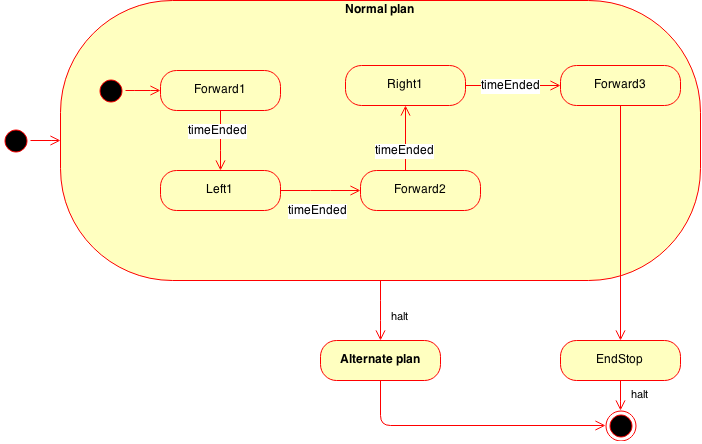
\includegraphics[scale=0.6]{img/ISS-robotStep1-FSM.png}


\subsection{Abstraction gap}

% PHYSICAL ROBOT CONFIGURATION ===> robotBase

Our \textbf{technology hypothesis} is given by 

\begin{itemize}
  \item our stack of custom frameworks,
  \item the Base Robot DDR DSL, and
  \item the High Robot DDR DSL
\end{itemize}


The problem and the practical issues encountered through the analysis phase
pointed out a gap exists in many themes/areas, namely:


\begin{itemize}
  \item \textbf{Model specification}: we have the need to build models of the
  system ($\Rightarrow$ S-I-C) that are \emph{formal}, at \emph{the
  right level of abstraction}, consistent, and easily modifiable.
  
  \item \textbf{General system concepts}: our systems approach should be
  supported by high-level concept such as ``environment'', ``context'', ``situated entity'',
  ``named entity'', \ldots 

  \item \textbf{Rapid prototyping}: we have the goal to have analysis end up
  with a working prototype that allows us to receive early feedback
  
  \item \textbf{Communication and interaction}: we have the need to express how
  our system entities interact in a high-level, technology-independent manner
  
  \item \textbf{Infrastructure configuration and setup}: we don't want to be
  concerned in the details of the system setup and configuration
  
  \item \textbf{Robot configuration}: we want to
  be able to easily specify the logical and physical configuration of a 
  robot  

  \item \textbf{Robot behavior and interaction}: we want to be able to specify
  	what a robot should do, perceive, react \ldots in a technology-independent manner

\end{itemize}

  After repeated interactions between application designers and system
  designers, our frameworks/DSLs have evolved to minimize the aformentioned gap
  between the problem and the execution platform.
 
 

\subsection{Risk analysis}

% A risk is any uncertain event or condition that might affect your project.
% An uncertainty that does not affect an objective is not a risk


 In addition to
 
 \begin{itemize}
   \item the possibility of changes in functional requirements (i.e., what the
   robot system should do)
   \item the possibility of changes in non-functional requirements (i.e., what
   properties the robot system should exhibit)
   \item the technological evolution (both hardware and software) in this very
   field
 \end{itemize} 
 
 which are more facts than uncertain events, we need to monitor and control the 
  following risks.
  
 \subsubsection{Performance and efficiency}
 
 Even though we do not have real-time requirements, it's important to realize
   that design decisions might seriously impact on performance, possibly
   resulting in significant delays (e.g., in the execution of reactions to
   events).
   
  \subsubsection{Distribution issues}
  
 From distribution, many issues arise:
 
\begin{itemize}
  \item Unreliability of the network
  \item Latency
  \item Changes in topology
  \item Security
  \item \ldots
\end{itemize}

  These potential problems need to be taken into account if 
   the robot is intended to be a \emph{dependable} system (i.e., available,
   reliable, safe, maintainable).

\subsubsection{Etherogeneity}
  
In the real world, these kinds of systems may be implemented using many
  different (hardware and software) technologies.
 
As a consequence, integration and interoperability issues may occur. 
  
%Hardware components may be different, possibly using low-level, ad-hoc
%communication protocols. Moreover, the software used to drive sensors/actuators 
% can be written in a different language with respect to the software that
 

\subsubsection{Testing and debugging}

Because of the many layers -- from the physical layer to the
 application layer -- and the many components involved, it might be difficult to
 trace and locate faults in case of errors.




%===========================================================================
\section{Work plan}
\labelsec{wplan}
%===========================================================================

\mybox{This section is related to the \textbf{product backlog} notion of 
the Scrum process framework.}

The team consists in 3 team members with cross-functional skills (analysis,
testing, implementation).

As we are following an iterative process, the work plan consists 
 in iterations with the following activities (not all of them necessarily
 executed at each cycle):
 
\begin{enumerate}
  \item Individual requirement analysis
  \item Requirement analysis: discussion and results
  \item Domain modelling
  \item Individual problem analysis
  \item Problem analysis: discussion and results
  \item Logic architecture refinement
  \item Risk analysis and work plan refinement 
  \item Abstraction gap evaluation
  \item Collaboration with system designers
  \item Implementation of application-specific parts
  \begin{itemize}
    \item \ldots (see next)
  \end{itemize}
  \item System integration testing
  \item User-acceptance testing
\end{enumerate}

These activities can be broke down into sub-tasks or address specific parts of
the artifacts involved. For example, as in this case study the requirements are
split into two parts, it has been natural to split the analysis activities
accordingly.

The work is parallelized when possible, however the results from analysis have
to be agreed on by all the team members. \\

Supposing we had to design/implement the system without the DSL (possibly before
building the DSL), the (high-level) work plan would have been something as:

\begin{itemize}
  \item \textbf{Base robot}: Design/implement a software system with a base
  robot that merely executes commands
  \item \textbf{Base robot + console}: Design/implement a software system with a
  base robot that merely executes commands sent by a remote console
  \item \textbf{Get sensor data}: Design/implement a software system that shows
  data from the robot's sensors
  \item \textbf{Autonomous, planned robot}: Design/implement a software system
  with an autonomous robot that executes its built-in plan
  \item  \textbf{Reactive/proactive robot}: Design/implement a software system
  with an autonomous robot that, while it executes its built-in plan, is able to react to sensor or application
  events
  \item \ldots
\end{itemize}

Note how the approach to development is incremental.

%The project team consists of three engineers. So, ideally, the work is
%subdivided on a subsystem-basis:

%\begin{itemize}
%  \item One developer will design/develop the Android subsystem
%  \item One developer will design/develop the RaspberryPi subsystem
%  \item One developer will design/develop the Arduino subsystem
%\end{itemize}

%Here, it is important to clearly define the subsystems' interfaces
%(communication media, communication language, \ldots). An architectural design
%will be defined (see Section \ref{sec:Project}) to better specify the
%constraints and interactions.

%Moreover, certain code/naming conventions should be defined in order to
% preserve the internal quality (coherence) of the system.




%===========================================================================
\section{Design}
\labelsec{Design}
%===========================================================================

The design of the system is encaspulated and enforced by the software
  factory of the DDR DSL (i.e., the code generators).
  
Please consult the DDR documentation (and ultimately the code generators) 
  to have the up-to-date, authoritative description of this aspect.

At the current version of the software factory, the following
\textbf{architectural style} is enforced:

\begin{itemize}
  \item Structural organization: \emph{contexts} populated by \emph{qactors}\\
  \texttt{robotsystemstep1.pl}
  \begin{lstlisting}
context(robotstep1, "localhost",  "TCP", "8020" ).  		 
context(userctx, "localhost",  "TCP", "8090" ).  		 

qactor( qactorconsole, userctx ).
qactor( robotActor, robotstep1 ).
\end{lstlisting}
  
  \item Interaction through \emph{messages}, \emph{events},
  \emph{streams of events}
\end{itemize}



%\begin{figure}[H]
%    \centering
%     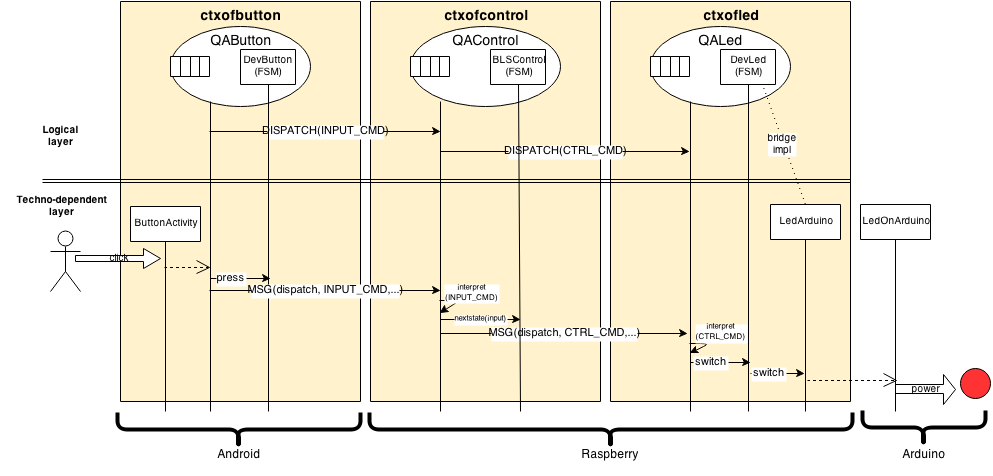
\includegraphics[scale=0.60, trim=4cm 0 0
%     -1cm]{img/BLSDesignArch-ActorBased.png}
%    \caption{Design architecture}
%    \label{fig:designarch}
%\end{figure}


%\subsection{Structure}
%\subsection{Interaction}
%\subsection{Behavior}


%===========================================================================
\section{Implementation}
\labelsec{Implementation}
%===========================================================================

The \textbf{schematic part} of the implementation of the system is generated 
from the logic architecture by the software factory, whereas the
\textbf{specific part} has to be implemented by the application designers.

\subsection{To be implemented}

The following pieces have to be implemented.

\subsubsection{Step1}


\begin{itemize}
  \item The event handler for \texttt{Line} events
  \item The QActor for the remote console
\end{itemize}

\subsubsection{Step2}

In addition to Step1:

\begin{itemize}
  \item The event handler for \texttt{Distance} events
\end{itemize}

%The design of the system is encaspulated and produced by the software
%factory of the DDR DSL (i.e., the code generators).

% See \emph{it.unibo.group08.buttonled.logical} and 
% \emph{it.unibo.group08.buttonled.actorsystem} projects.



\subsection{On the robot implementation}

The robot subsystem is a context (\texttt{ActorContext}). Its setup consists
in:

\begin{itemize}
  \item Setup of the robot \texttt{QActor}
  \begin{itemize}
    \item Loading of the robot configuration (\texttt{robotConfig.properties},
    \texttt{hardwareConfiguration.properties},
    \texttt{iotRobot.properties})
    \item Configuration of the base robot and its components
    \item Launch of the robot
  \end{itemize}
  \item Creation of the event handlers / tasks
  \item Loading of \texttt{WorldTheory.pl} as a TuProlog theory
  \item Setup of the USB connection and/or the HTTP server
  \item Setup of the observers for sensors and registration of the subscribers
  \item Setup of the Nashorn JS Engine, loading of the JavaScript robot
  interpreter, and execution of the plans
\end{itemize}


%===========================================================================
\section{Testing}
\labelsec{testing}
%===========================================================================

The testing activities are usually carried out in the following order:

\begin{enumerate}
  \item \textbf{System integration testing: robot mock, concentrated
system} \\
\quindi{This step allows us to assess the application logic
	without incurring in deployment/network/technology issues.}

\item \textbf{System integration testing: robot mock, distributed system} \\
\quindi{Let's add one big concern at a time, here distribution.}

\item \textbf{System integration testing: physical robot}\\
\quindi{Deployment testing}

\item \textbf{User acceptance testing} (simulated)\\
\quindi{Is the software right? Is what the user/customer expects?}

\end{enumerate}

\mybox{The \textbf{robot mock} is extremely useful because it allows to test the
system without the need to deploy it into a physical robot (which demands
resources to be built and may require significant effort for deployment and
	configuration activities). }


% See \emph{it.unibo.group08.buttonled.test} project.




%===========================================================================
\section{Deployment}
\labelsec{Deployment}
%===========================================================================

 The requirements do not specify any particular deployment configuration.
 
 An example configuration is the following one:
 
 \begin{itemize}
   \item ROBOT: A JAR package for the RaspberryPi subsystem that commands the
   physical robot
   \item USER CONSOLE: A JAR package for the user console
 \end{itemize}
 
 The logic architecture expressed using the HighRobot DDR DSL includes
 deployment details, but they could also be changed in the generated artifact
 	\texttt{robotsystem.pl} which contains the declarations of the contexts
 	(subsystems) of the system.
 

%===========================================================================
%\section{Maintenance}
%\labelsec{Maintenance}
%===========================================================================



\newpage

%===========================================================================
\section{Discussion}
\labelsec{Discussion}
%===========================================================================

\subsection{UML vs. Java interfaces + test plans vs.
Metamodelling}

As outlined in the Section \emph{Vision}, we are for using the right tool at the
right time and for the right purpose.

When we are modelling, we want to come up with models that are unambiguous,
formal, at the right level of abstraction, human-understandable. These models 
 should also be kept consistent with related artifacts with little pain.

When using \textbf{UML}, we encounter many issues:

\begin{itemize}
  \item UML models can be read by tools (i.e., the syntax of UML is
    well-defined), but the semantics of UML is \textbf{ambiguous} to some
    extent (it suffices to say that UML elements are described in natural language -- inherently ambiguous)
  \item As a result, the \textbf{semantics} of UML is that given by a certain
  UML tool -- but we are not guaranteed that the representations of our models are
    interoperable among different tools, nor against different versions of the
    same tool ($\Rightarrow$ risk of \emph{vendor lock-in} and \emph{version
    lock-in})
  \item While possible, it is not (technically) easy to keep UML models
  \emph{in-synch} with source code
  \item The \textbf{generation of code} from UML diagrams presents many issues
  as well.
  UML diagrams are useful when they abstract implementation details out of the
  actual code. On the other hand, a diagram which is easy to understand turns
  out to be not very useful for code generation; moreover, in this case, the
  code itself does the job nicely.
  \item Not everything can be \emph{expressed} with UML. We, throughout the ISI
  course, have found ourselves in extending UML with ad-hoc notations.
  UML is quite related to the object-oriented paradigm, but we might find 
  \textbf{expressivity} issues when we are out the OOP realm.  
\end{itemize}

However, UML still represents a useful, standard communication tool in many
situations. \\

The use of \textbf{Java interfaces} for modelling is an approach for doing
analysis while actually writing code at the same time. For us, a Java interface
represents a model of a domain concept. However, while formal, they are merely
syntax; their semantics is just in our minds (implicit in our convention). To
better specify the semantics of the concepts modelled through interfaces, we 
write \textbf{test plans} (which will also work as (regression) tests once
implementation classes are built). \\

As long as the concepts can be easily expressed through the Java
metamodel, this approach works well. Howerver, what can we do in case of
expressivity issues, unappropriate level of abstraction, modelling
mismatch, \ldots? We also note that these analysis artifacts are not very
technology-agnostic..

Another approach consists in developing a \textbf{custom meta-model} that
 gives names to (domain) concepts and defines the abstract syntax of
 a (custom, technology-independent) modelling language. Then, it is possible to
 specify (custom) semantics by defining \emph{model transformations}.

% When msg. passing?

\subsection{Meta-model as a living artifact} 

We note that the meta-model has an \textbf{evolving nature}.

 In fact, as long as we get a better comprehension of the problems and the
  applications generate \emph{forces} that stress the \emph{expressive power} of
  the metamodel, we might found ourselves in the need of
  refactoring/extending/changing the metamodel.
    
\subsection{A DSL is a project!}

The DSL should be considered a software project on its own. 
  Requirements come from applications and the feedback from application
  designers. The requirements and the problem have to be analyzed:
  what has to be expressed with the DSL? what levels of abstraction are
  required? are there trade-offs between expressivity and performance? \ldots 
  The language abstract and concrete syntaxes have to be properly designed as
  well as the code generators. There are multiple (often conflicting) design
  dimensions (such as expressivity, domain coverage, semantics, separation of
  concerns, completeness for execution, language modularization, syntax \cite{dsleng}) to
  be taken into account.


\subsection{Agile (Scrum, \ldots) vs. MDSD}

We essentially agree with the principles behind the Agile Manifesto\cite{agile}
and its motto

\begin{itemize}
  \item \textbf{Individuals and interactions} over processes and tools
  \item \textbf{Working software} over comprehensive documentation
  \item \textbf{Customer collaboration} over contract negotiation
  \item \textbf{Responding to change} over following a plan
\end{itemize}

 however we note that they are essentially ``defining'' principles
that say little about their actualization. Agile tends to be \emph{descriptive}
 rather than \emph{prescriptive} (with exceptions, cf. XP), but this results in
 a gap from theory to execution. As a consequence, Agile is often
 misunderstood/misapplied.

Concerning the \textbf{Scrum} process framework, we recognizes that it may help
the projects by forcing people to perform short iterations (cf. sprints,
early feedback) and take good habits (cf. the \emph{product backlog} as the
unique list of things to do, \emph{retrospectives}, fostering
\emph{incremental development}, avoid over-engineering by limiting the work-in-progress in the
\emph{sprint backlog}, the \emph{scrum master} as a facilitator \ldots).
However, there are many other degrees of freedom that might make 
 the projects fail (c.f., self-organizing teams).
 
$$\\$$
 
We do not see any significant contradiction between Agile and MDSD that would
  make them irremediably incompatible.

Historically, agile has always been for building the real
  system as soon as possible in order to get early feedback, while at the same
  time avoiding over-specification. Whereas there is the myth that
  model-driven approaches must be necessarily heavyweight.

We think that a fruitful link between Agile and MDSD can exist because:

\begin{itemize}
  \item Coding is not fundamentally different from modelling
  \item Models can be developed iteratively and incrementally
  \item The distance between models and the final system can be reduced via code
  generators 
\end{itemize}

%http://modeldrivensoftware.net/forum/topics/why-modeling-and-code

$\\ \\$

\subsection{On the relationships between the DSL and the technological
infrastructure}

\subsubsection{Many layers}

 The system we have built can be seen as a \emph{layered} system.

\begin{figure}[H]
    \centering
     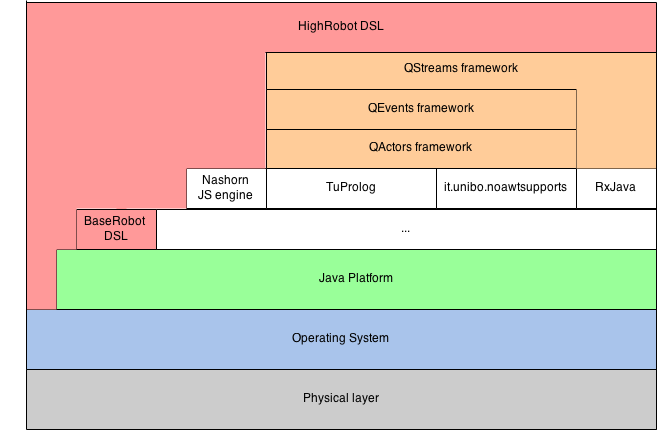
\includegraphics[scale=0.68, trim=4cm 0 0
     -1cm]{img/ISS-Layers.png}
    \caption{Layers.}
    \label{fig:layers}
\end{figure}

The \emph{layered} approach (or, the Layers
architectural pattern \cite{posa1}) 
is an application of the \emph{divide-et-impera} principle and is good for reducing complexity and fostering simplicity and
  order. In fact, the dependencies of a single piece (layer) are reduced to just
  the layers directly below.
  
In our experience, we have seen how this approach  \textbf{supports a
 sustainable, gradual, step-by-step reduction of the abstraction gap} and
 fosters a modularization that turns out to be very good for reuse.
  

\subsubsection{Integrating top-down and bottom-up approaches: a hybrid
approach}

 We have experienced the advantages and the \emph{theoretical} reason behind
  following a top-down approach.
 
 However, the \emph{pragmatical} issues encountered (during implementation)
 often require to cope with technological details in order to make things work 
  or to get a sense of some aspects of the problem at hand. Moreover, for
  example, it is possible that theoretically irreproachable solutions 
  could result in inappropriate actualizations (e.g., because of the
  limitations and constraints of the available underlying technology). 

 Thus, \textbf{a bottom-up approach can be combined to a general top-down
 attitude in order to get a quicker feedback on technological issues, identify unforeseen 
  problems that might emerge at higher levels, or identify relevant features
  not included in the models}.
  
 Our idea, when there are mutual influences among upper and lower layers, is not
 to be dogmatic or biased, but to be flexible 
 and able to evaluate the pros and cons of each decision/alternative.

 This discussion recalls to the relationship \emph{between theory and practice}.
   They are correlated; a tension exists between them. 
   We suggest to be balanced: to make practice with theoretical foundations,
   and to make theory with cognition/feedback from practice.

% ABSTRACTIONS AND TRADE-OFFS
% ISSUES OF ABSTRACTION

\subsubsection{Abstraction, issues and trade-offs}

 Abstraction is not free. It has a cost, and when 
  abstractions are designed, that cost has to be considered.
 We remember that engineering is also about making trade-offs.
 
 Models should specify enough details to be useful. In some cases,
  implementation details should be provided (anticipated) in order to generate
  architectures that fit the concrete, specific application scenario (e.g., for
  performance or security).


\subsubsection{More on the DSL and layers}  
  
  The robot is a QActor because it is active (and autonomous) and lives in a
  distributed setting where message-passing is a convenient communication style.
  Why have we chosen to make it a QActor rather than a lower-level (e.g.,
  active objects) or higher-level (e.g., agents) abstraction?
  For the first case, we would have experienced a significant effort in trying
  to fill the abstraction gap; about the second option, we note that 
  agent abstractions typically include higher-level characteristics that 
  are unneccessary or too complex at the present time, not (yet) motivated by
  analysis.
  
  About the contexts (our subsystem abstraction), we note that they have been 
   included as part of the HighRobot DSL (up to version 1.1.8, with an
   '\texttt{ActorContext}' keyword) and directly map to QActors'
   \texttt{ActorContext}s. The DSL also supports the declaration of actors
   within the declared contexts. This is an example of lower-level concepts 
   that are pushed up to the DSL level not only for simplicity and rapid
   prototyping needs but also because of information needs in the 
   code generation phase.

 Similarly, the HighRobot DSL also includes keywords such as \texttt{-http} and
 \texttt{-usb} to activate an HTTP web server and a USB connection,
 respectively. This is another example (concerning the theme of DSL and
 software factory design) of technology details that are anticipated for
 practical issues.
   
 


%\begin{itemize}
%  \item Early and continuous delivery of valuable software to satisfy the
%  customer \\
%  \quindi{cf. prototyping, iterative process, piecemeal growth
%  development}

%  \item Welcome changing requirements, even late in development \\
%  \quindi{cf. reuse, domain modelling, sustainable reduction of
%  abstraction gap (layered approach)}
  
%  \item Deliver \emph{working} software frequently \\
%  \quindi{cf. iterative process, piecemeal growth development}
  
%  \item Business people and developers must work together daily throughout the
%  project \\
%  \quindi{cf. early feedback, analysis \& domain modelling, DSL,
%  application designers and system designers}
  
%  \item Build projects around motivated individuals. Give them the environment
%  and support they need, and trust them to get the job done \\
%  \quindi{cf. human factors in software projects} \cite{peopleware}
  
%  \item The most efficient and effective method of conveying information to and
%  within a development team is face-to-face conversation \\
%  \quindi{OK but should be supported by explicit, unambiguous artifacts (e.g.,
%  models); otherwise, there's the risk that a lot of knowledge is kept
%  hidden (implicit)}
  
%  \item Working software is the primary measure of progress \\
%  \quindi{cf. analysis effort capitalization, prototyping, piecemeal growth
%  development}  

%  \item Agile processes promote sustainable development (ability to keep
%  constant pace indefinitely) \\
%  \quindi{How?}
  
%  \item Continuous attention to technical excellence and good design \\
%  \quindi{cf. refactoring, patterns, reuse, technical debt reduction}
  
%  \item Simplicity is essential
%  \item The best architectures, requirements, and designs emerge from
  % self-organizing teams
%  \item At regular intervals, the team reflects on how to become more
  % effective, then tunes and adjusts its behavior accordingly
%\end{itemize}



%\newpage
%See \cite{natMol09} until page 11 (\texttt{CMM}) and pages 96-105.

%===========================================================================
\section{Information about the authors}
\labelsec{Author}
%===========================================================================

\vskip.5cm
%%% \begin{figure}
\begin{tabular}{ | c | c | c |  }
\hline
  % after \\: \hline or \cline{col1-col2} \cline{col3-col4} ...
   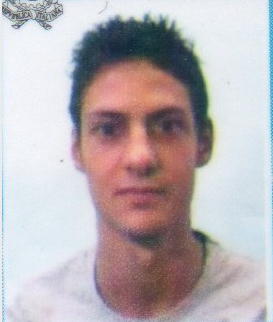
\includegraphics[scale = 0.4]{img/fototessera.jpg}
   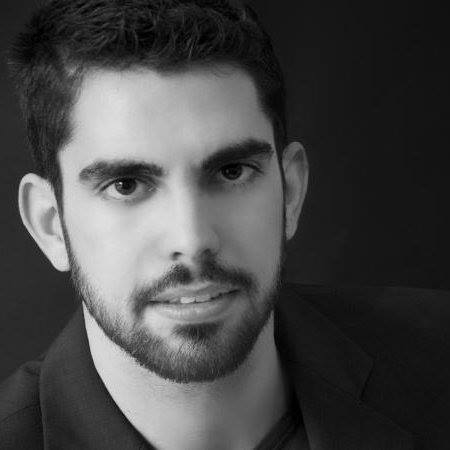
\includegraphics[scale = 0.25]{img/reda.jpg}
   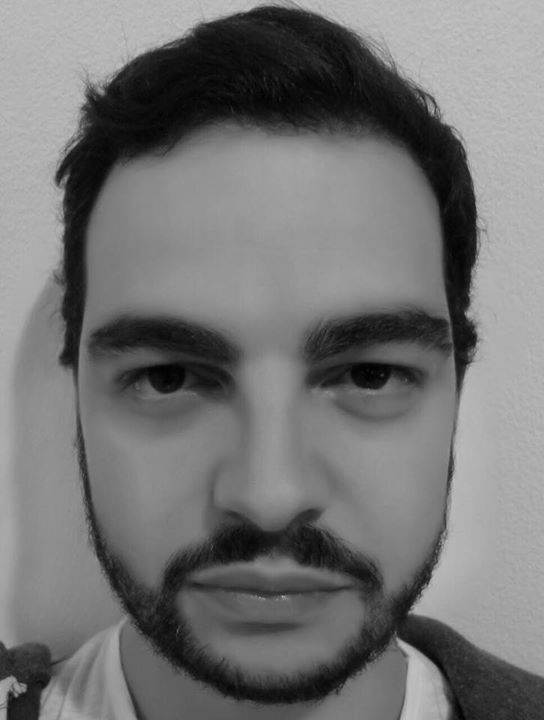
\includegraphics[scale = 0.18]{img/martella.jpg}
\end{tabular}


%%% \begin{itemize}
%%% \item Titolo di studio:\\ \\
%%% \item Interessi particolari:\\ \\
%%% \item Ha sostenuto fino ad oggi il seguente numero di esami:\\ \\
%%% \item Deve ancora sostenere i seguenti esami del I anno:\\ \\
%%% \item Prevede di svolgere un tirocinio presso:\\ \\
%%% \item Prevede di laurearsi nella sessione:\\ \\
%%% \item Intende proseguire gli studi per conseguire: \\  \\  \\
%%%   	presso la sede universitaria di: \\ \\
%%% \item Intende entrare subito nel mondo del lavoro presso : \\ \\
%%% \end{itemize}

 
\appendix

\nocite{gof94}
\bibliographystyle{abbrv}
\bibliography{biblio}

\end{document}

